% vim: ts=2 sts=2 sw=2

\documentclass[a4paper,12pt]{report}
\usepackage{a4wide}
\usepackage[finnish]{babel}
\usepackage[utf8]{inputenc}
\usepackage[T1]{fontenc}
\usepackage{graphicx}
\usepackage{float}

\title{
\includegraphics[width=5em]{logo}\\\vspace{1em}MusicGhost\\\vspace{1em}
  \large{Tietokantasovellus, kevät 2011\\Tietojenkäsittelytieteen
  laitos\\Helsingin yliopisto}\\}
\author{Tuomo Lempiäinen\\\texttt{tuomo.lempiainen@helsinki.fi} \and
Hanna Nieminen\\\texttt{hanna.m.nieminen@helsinki.fi}}

\begin{document}

\maketitle

\tableofcontents

\chapter{Määrittely}

\section{Johdanto}

\subsection{Järjestelmän tarkoitus}
Järjestelmän avulla sen ylläpitäjä voi pitää kirjaa levykokoelmastaan.
Järjestelmä tarjoaa useita erillisiä listoja, jolloin on mahdollista
erotella esimerkiksi omistamansa levyt ja tulevat hankinnat toisistaan.
Järjestelmästä voi tehdä julkisen, jolloin myös vierailijat voivat selata
levylistaa ja yksittäisten levyjen tietoja.

\subsection{Toimintaympäristö}
Järjestelmää käytetään WWW-selaimen kautta. Sen ajamiseen tarvitaan
Apache-palvelin varustettuna PHP5-tuella sekä PostgreSQL-tietokanta.

\subsection{Rajaukset}
Kaikki ominaisuudet, joita ei ole tässä määrittelyssä erikseen mainittu, on
oletusarvoisesti rajattu järjestelmän ulkopuolelle.

\subsection{Toteutusympäristö}
Järjestelmän toteuttamisessa hyödynnetään Vim-editoria Arch Linux
-käyttöjärjestelmässä sekä Notepad++-editoria Windows 7
-käyttöjärjestelmässä. Toteutuksen aikana järjestelmää testataan
paikallisilla Apache- ja PostgreSQL-palvelimilla.

\section{Yleiskuva järjestelmästä}

\subsection{Sidosryhmäkaavio}

\vspace{1em}
\begin{figure}[H]
  \begin{center}
    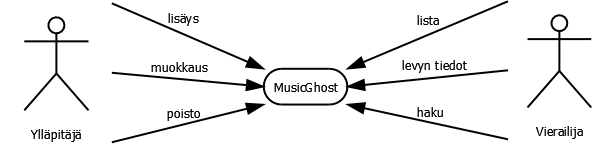
\includegraphics[width=\textwidth]{diagrams/sidosryhmakaavio}
  \end{center}
  \caption{Sidosryhmäkaavio}
\end{figure}

\subsection{Käyttäjäryhmät}
\begin{description}
\item[Vierailija] Kuka tahansa sivulla vieraileva käyttäjä. Myös tietokannan
omistaja kuuluu tähän luokkaan.
\item[Ylläpitäjä] Levytietokannan omistaja,
joka ylläpitää tietokantaa.
\end{description}

\section{Käyttötapaukset}

\begin{itemize}

\item Vierailija:
\begin{description}
\item[Levylistan selaaminen] Kuka tahansa voi katsella tietokannan sisältöä.
Listauksessa näkyy kunkin levyn kohdalla sen esittäjä, nimi, julkaisuvuosi ja
formaatti.
\item[Yksittäisen levyn tietojen tutkiminen] Käyttäjä voi valita yksittäisen
levyn, jolloin hänelle näytetään kaikki siihen liitetyt tiedot.
\item[Levyjen hakeminen hakusanalla] Käyttäjä voi antaa hakusanan, jolloin
hänelle näytetään lista niistä levyistä, joiden tiedot sisältävät annetun
hakusanan.
\item[Kirjautuminen sisään] Mikäli vierailija sattuu olemaan tietokannan
omistaja, hän voi kirjautua sisään järjestelmään, jolloin hänestä tulee
ylläpitäjä.
\end{description}

\item Ylläpitäjä:
\begin{description}
\item[Levyn lisääminen] Ylläpitäjä voi lisätä uusia levyjä tietokantaan.
Ylläpitäjä syöttää ainakin levyn tyypin, esittäjän ja nimen sekä valitsee, mille
listalle se lisätään. Vapaaehtoisia tietoja ovat levyn julkaisuvuosi, formaatti,
kansikuva ja vapaamuotoinen kommentti. Esittäjäksi voi valita listasta jonkin jo
tietokannasta löytyvän esittäjän tai vaihtoehtoisesti syöttää kokonaan uuden.
\item[Levyn tietojen muokkaaminen] Ylläpitäjä voi muokata kaikkia yksittäiseen
levyyn liitettyjä tietoja.
\item[Levyn poistaminen] Ylläpitäjä voi poistaa levyn tietokannasta.
\item[Kirjautuminen ulos] Ylläpitäjä voi tarvittavat ylläpitotehtävät tehtyään
kirjautua ulos, jolloin hänestä tulee vierailija.
\end{description}

\end{itemize}

\chapter{Suunnittelu}

\section{Järjestelmän tietosisältö}

\begin{figure}[H]
  \begin{center}
    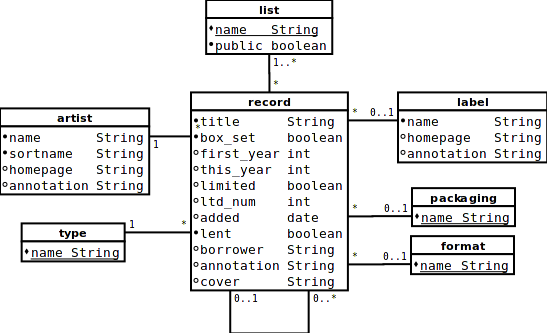
\includegraphics[width=0.8\textwidth]{diagrams/kasitekaavio}
  \end{center}
  \caption{Käsitekaavio}
\end{figure}

\begin{itemize}
\item record
\begin{description}
\item[box\_status] Onko kyseessä normaali levy, boksi vai boksiin kuuluva levy?
\item[type] Levyn tyyppi -- esimerkiksi albumi, single tai live.
\item[first\_year] Levyn ensimmäinen julkaisuvuosi.
\item[this\_year] Kokoelmassa olevan levyn julkaisuvuosi.
\item[limited] Onko levy rajoitettua painosta?
\item[ltd\_num] Rajoitetun painoksen painosmäärä.
\item[added] Päivä, jolloin levy on lisätty kokoelmaan.
\item[lent] Onko levy lainassa?
\item[borrower] Henkilö, jolle levy on lainattu.
\end{description}
\end{itemize}

\section{Käyttöliittymän hahmotelma}

\begin{figure}[H]
\begin{center}
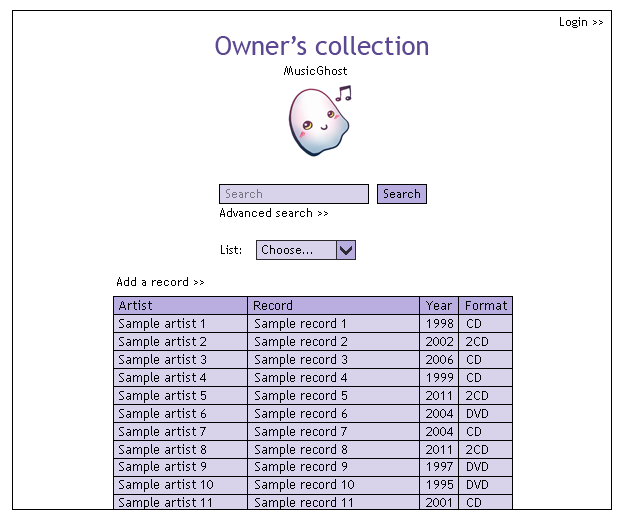
\includegraphics[width=\textwidth]{mainwindow2}
\end{center}
\caption{Etusivu}
\end{figure}

\begin{figure}[H]
\begin{center}
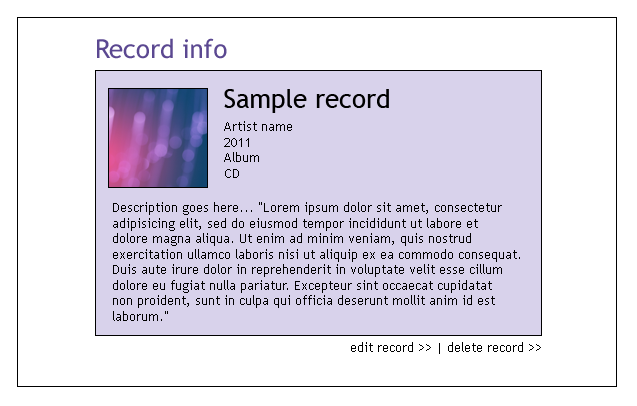
\includegraphics[width=\textwidth]{recordinfopage}
\end{center}
\caption{Levyn lisätietosivu}
\end{figure}

\begin{figure}[H]
\begin{center}
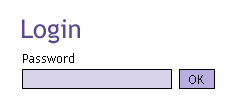
\includegraphics[]{login}
\end{center}
\caption{Kirjautuminen sisään}
\end{figure}

\begin{figure}[H]
\begin{center}
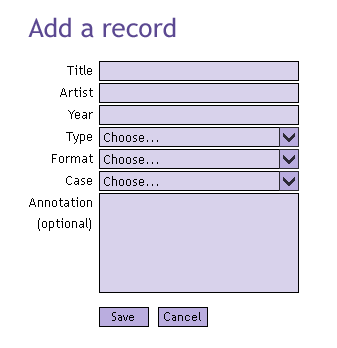
\includegraphics[]{addpage}
\end{center}
\caption{Levyn lisääminen}
\end{figure}

\begin{figure}[H]
\begin{center}
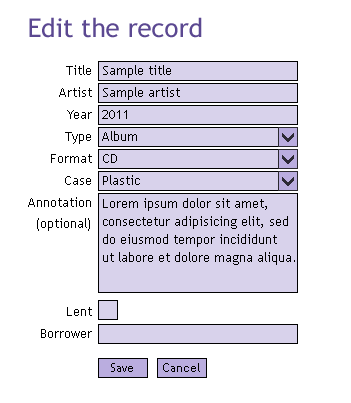
\includegraphics[]{editpage}
\end{center}
\caption{Levyn muokkaaminen}
\end{figure}

\begin{figure}[H]
\begin{center}
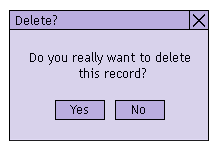
\includegraphics[]{delete}
\end{center}
\caption{Levyn poiston varmistusdialogi}
\end{figure}

\section{Relaatiotietokantakaavio}

Relaatiotietokantakaavio on esitetty \texttt{CREATE TABLE} -lauseina tiedostossa
\texttt{create\_tables.sql}.

\end{document}
